\section{The CQF Hashing Extension}
The hash study changes the path that maps an original key to a CQF fingerprint while keeping table geometry, stream order and remainder width fixed within each comparison. The CQF's slot layout, metadata and counter representation are unchanged. This lets us test an engineering alternative without presenting an existing mixer as a new hashing algorithm.

\begin{figure}[!htbp]
\centering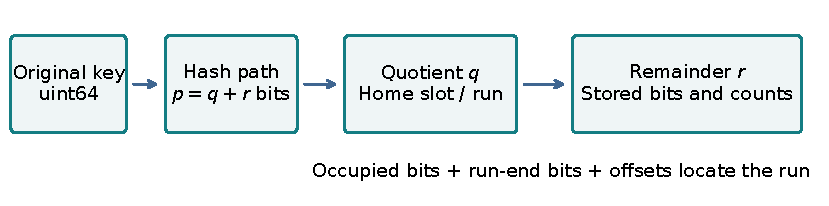
\includegraphics[width=0.94\linewidth]{cqf_layout.pdf}
\caption{Conceptual CQF path. Hashing, table geometry and counting are separate choices. The diagram illustrates the representation; it is not a memory dump of a measured run.}
\label{fig:cqf-layout}
\end{figure}

\subsection{Three end-to-end paths}
\begin{table}[!htbp]\centering\small
\caption{Hash paths evaluated with $p=q+r$ fingerprint bits. The external mixer is recomputed inside every timed insert, query and deletion loop.}
\label{tab:hash-paths}
\begin{tabular}{L{2.25cm}L{6.4cm}L{4.1cm}}\toprule
\textbf{Driver mode}&\textbf{Mapping before CQF run access}&\textbf{Cost included}\\\midrule
\texttt{default}&$\mathrm{MurmurHash64A}(x,\mathrm{seed}=0)\bmod 2^p$&Internal key hashing and CQF operation\\
\texttt{invertible}&Reference Thomas Wang integer mixer restricted to $p$ bits&Internal integer mixing and CQF operation\\
\texttt{none}&$\mathrm{SplitMix64}(x)\;\&\;(2^p-1)$, then \texttt{QF\_HASH\_NONE}&External mixing and CQF operation\\\bottomrule
\end{tabular}
\end{table}


Each path uses the same mapping for insertion, successful queries, negative queries and deletion. Precomputing this external hash outside the timed loop would remove work paid by the other modes. We explicitly include it. Therefore \texttt{none} means that the CQF performs no additional internal hash, not that the experiment has no hashing cost.

\subsection{What invertibility does and does not mean}
The reference invertible mixer is a permutation of the configured $p$-bit domain. That property does not preserve all original keys here: our integer inputs span a wider domain than $p=29$ in the 996k control or $p=36$ at 67M. The path projects keys into a smaller domain, where different original keys can collide. It must not be described as collision-free or as giving zero FPR. The external SplitMix64 path also loses information when masked to $p$ bits, despite using a full-width mixer first.

The default CQF path reduces modulo a runtime range stored as a 128-bit integer, whereas our external path uses a direct mask for its power-of-two domain. Thus range reduction and API-path work are part of the comparison, not just the mixer arithmetic. Both geometry and hash path affect the addresses touched by CQF operations. Consequently, a change in end-to-end throughput can reflect instruction cost, changed fingerprint collisions and changed run access, rather than pure hash-function latency. We make no standalone hash-cycle claim and no cryptographic or adversarial-input claim.

\subsection{Controlled experiment matrix}
Further source-level details for both internal mappings are given in Appendix~\ref{app:hash-details}. We run all three modes on both distributions with three timing repetitions and 10M negatives. The 996,148-operation control uses $q=20,r=9$ and includes occurrence-by-occurrence deletion. The 67M study uses $q=27,r=9$ and measures insertion and both query classes; deletion is omitted there by design. Large-scale deletion is still measured in the seven-filter comparison. Memory is identical across modes at a fixed scale. This isolates the hash-path choice within that configuration, while the change of $q$ prevents treating the two scales as one pure hash microbenchmark.
\clearpage
